%04chapterFremdeinsch.tex
\chapter{Fremdeinschätzungen}\label{Fremdeinschaetzung}
Nach unseren individuell erstellten Selbsteinsch"atzungen, folgen nun die Fremdeinsch"atzungen, welche f"ur
den Vergleich von Selbst- und Fremdbild unabdingbar sind.
Dazu hat jedes Teammitglied seine eigene Form der Bearbeitung gew"ahlt. Dies war einerseits der Selbsteinsch"atzungstest, andererseits wurden anhand von spezifisch beobachteten Situationen eine Teamrollenzuteilung
vorgenommen.
\subsection*{Pascal Horat}

Auch um meine Teamkameraden einzuschätzen habe ich mich des vorher beschriebenen Belbin-Tests bedient. Dies vor allem aus drei Gründen:
\begin{enumerate}
\item Durch die vorgegebene Form ergibt sich meiner Meinung nach eine neutralere Betrachtung der Teamitglieder, da meine Einschätzung nicht nur auf ein bis zwei spezifischen Vorfällen beruht.
\item Durch die vorgegebene Form mit den Aussagen werde ich durch das Verfahren geleitet und muss nicht selber etwas entwickeln.
\item Da für die Bestimmung der Selbst- sowie der Fremdeinschätzung derselbe Test verwendet wurde, können direkte Vergleiche zwischen den Teammitgliedern gemacht werden.
\end{enumerate}

Dies hat für Gerome folgende Resultate hervorgebracht:


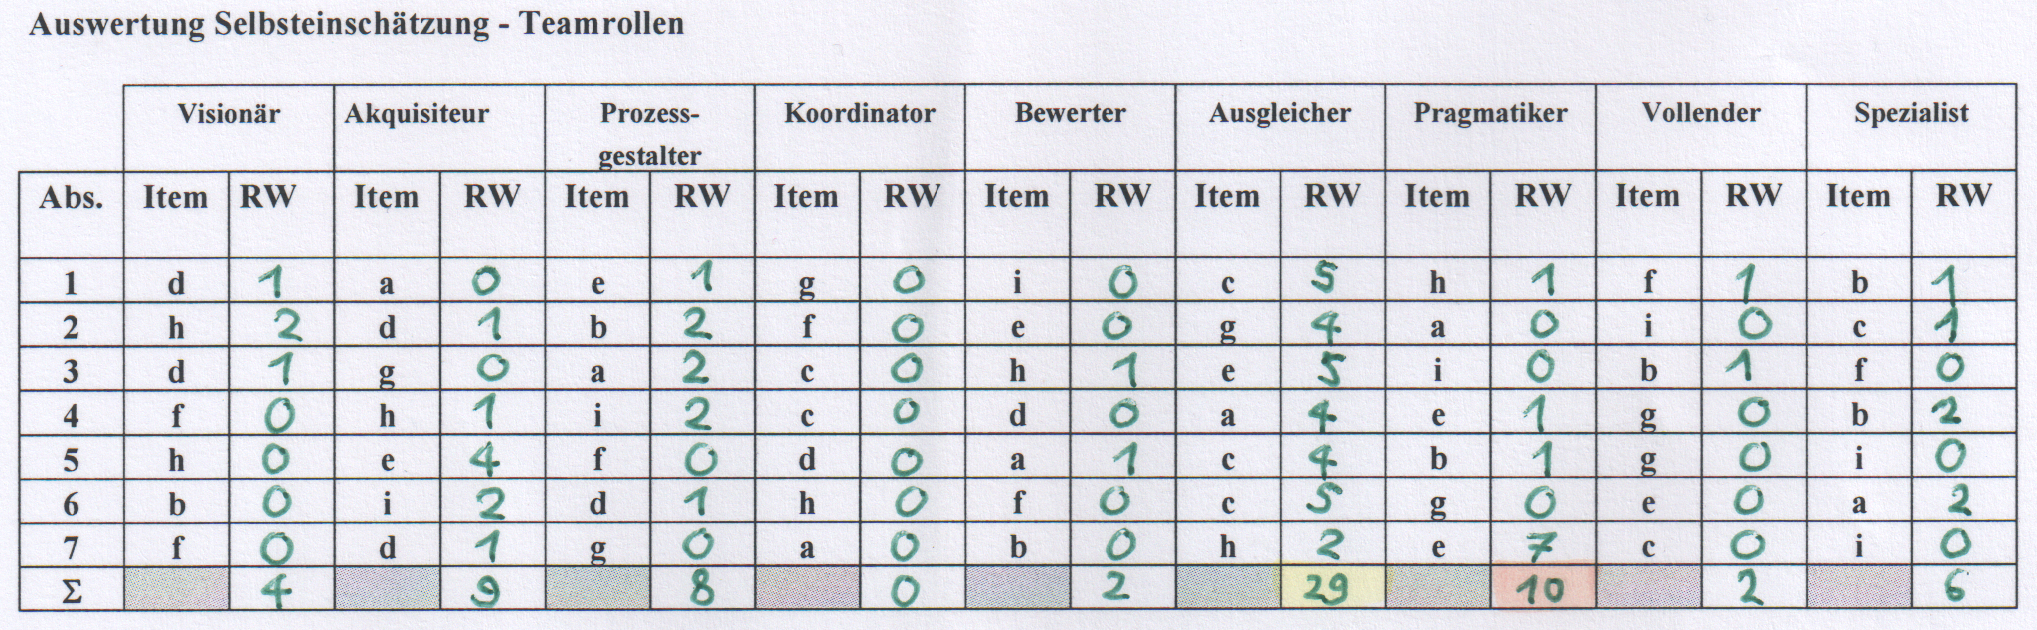
\includegraphics[height=39mm]{images/FremdeinschaetzungHoratKamga.png}

Von meinen Teammitgliedern fiel es mir, ohne die Hilfe des Tests, schwieriger, Gerome eine passende Rolle zuzuteilen. Darum hätte ich eine ausgeglichenere Punkteverteilung bei der Auswertung erwartet. Die Rolle des Ausgleichers, bei welcher er am meisten Punkte sammelte, finde ich jedoch passend. Dass sie bei ihm aber so ausgeprägt zum Zuge kommt, hat mich eher überrascht.

Bei Gökhan sieht die Auswertetabelle folgendermassen aus:

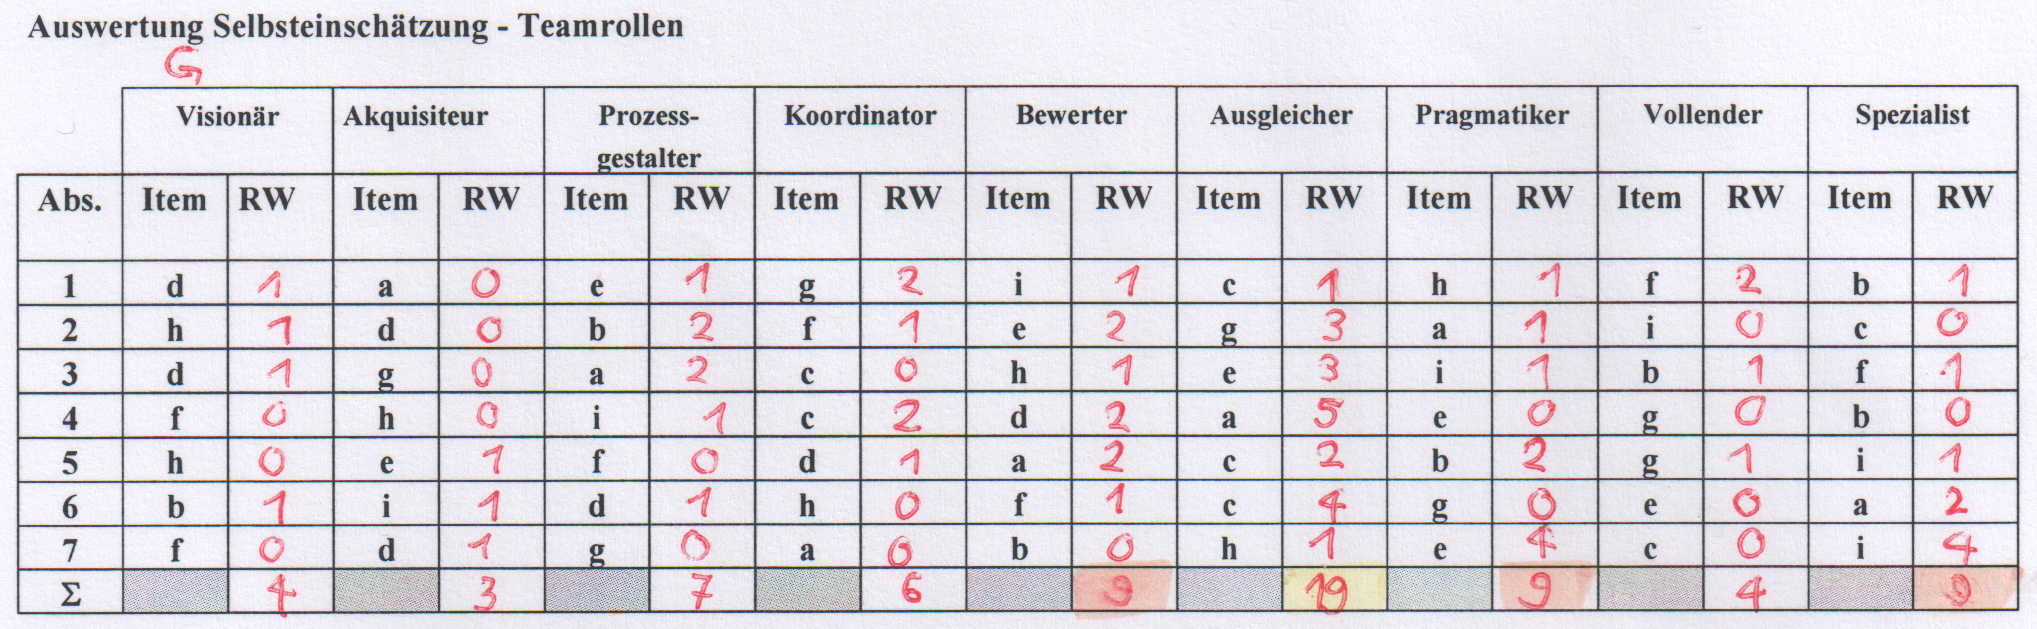
\includegraphics[height=39mm]{images/FremdeinschaetzungHoratKaya.png}

Bei ihm habe ich schon im Vornherein erwartet, dass er punktemässig eine Ausgleicher-Rolle erhalten würde. Interessanterweise war diese Rollenzuteilung aber viel ausgeglichener als vorher bei Gerome obwohl ich instinktiv eher das Gegenteil erwartet hätte. 

\subsection*{Steve Gerome Kamga}

Meine beiden Teammitglieder wurden auch von mir mit der Belbin-Methode eingeschätzt und die Ergebnissen werden folgendermassen dargestellt: \\
Nach meiner Einschätzung kam heraus, dass Pascal die nachfolgenden Rollen in einem Team übernehmen könnte:
\begin{enumerate}
\item Koordinator
\item Prozessgestalter
\item Bewerter
\end{enumerate}


Gökhan dagegen ist meiner Meinung nach mehr der:
\begin{enumerate}
\item Bewerter
\item Spezialist
\item Ausgleicher
\end{enumerate}


\subsection*{Gökhan Kaya}

Ich habe meine zwei Teamkollegen folgendermassen eingeschätzt:\\

Pascal war für mich der Koordinator und zwar aus den folgenden erlebten Gründen:
\begin{enumerate} 
\item{Meist sagt Pascal am Anfang der Sitzung was zu tun ist und gibt uns einen kleinen Überblick. Er ist somit sehr gut organisiert.}
\item{Er ist meistens der erste, der sich mit dem Dozenten in Verbindung setzt, wenn etwas noch unklar ist. Die nötigen Informationen leitet er uns anschliessend weiter.}
\item{Bereits bei der ersten Vorlesung ist mir aufgefallen, dass Pascal sich sehr vieles notiert und teilweise nach der Vorlesung ebenfalls mitteilt, was er sich notiert hat.}
\end{enumerate}

Gerome war für mich ganz klar der Vollender. Dies aus den folgenden drei Gründen:
\begin{enumerate} 
\item{Gleich nach der Teambildung konnte Gerome noch nicht auf moodle zugreifen. Er hat sich nach einem Tag bereits sofort gemeldet und mitgeteilt, dass bei ihm nun alles soweit funktioniert. Dies obwohl es nicht nötig gewesen wäre.}
\item{Ebenfalls hat nach der ersten Aufgabenteilung sofort auf WhatsApp geschrieben und uns mitgeteilt, dass er sein Auftrag erledigt hat. Pascal und ich empfanden dies hingegen als nicht nötig.}
\item{Als wir am letzten Tag vor der Abgabe noch bis spät die Lernbilanzen fertig gestellt haben, hat Gerome die ersten zwei Stunden ausschliesslich recherchiert, um das bestmögliche Produkt abzugeben. Dies obwohl wir nur wenig Zeit hatten. Dabei machte es ihm auch nichts aus, bis spät in die Nacht hinein zu arbeiten.}
\end{enumerate}
